\documentclass[14pt]{extarticle}
\usepackage{fontspec}
\usepackage{polyglossia}
\usepackage{amsmath}
\usepackage{amssymb}
\usepackage{xcolor}
\usepackage{fancyhdr}
\usepackage{graphicx}
\usepackage{listings}
\usepackage[most]{tcolorbox}
% \usepackage{setspace}
\usepackage{pifont}
\usepackage{enumitem}
\usepackage{titlesec}
\usepackage[bottom]{footmisc}
\usepackage{titling}
\usepackage{minted}
\usepackage{etoolbox}
\usepackage{array}
\usepackage{extsizes}
\usepackage{float}
\usepackage{booktabs}
\usepackage{hyperref}
\usepackage[onehalfspacing]{setspace}
\usepackage[a4paper, top=2.7cm, bottom=2.7cm, left=2.5cm, right=2.5cm, headheight=1.5cm, headsep=0.5cm]{geometry}
\usepackage{tikz}

\usetikzlibrary{automata, positioning, arrows.meta, arrows}

\newfontfamily\emoji{Segoe UI Emoji}

\pagestyle{fancy}

\setmainlanguage[numerals=western]{arabic}
\setotherlanguage{english}
% \newfontfamily\arabicfont[Script=Arabic]{Amiri}
\newfontfamily\arabicfont[Script=Arabic]{Calibri}
\newfontfamily\arabicfonttt[Script=Arabic]{Courier New}

\lstset{
  language=[Sharp]C,
  numbers=left,
  stepnumber=1,
  numbersep=8pt,
  frame=single,
  basicstyle=\ttfamily\small,
  keywordstyle=\color{blue},
  stringstyle=\color{red},
  commentstyle=\color{green!50!black}
}

\newif\ifdetailed
\ifdefined\setdetailed
  \setdetailed
\fi

\newif\ifwithsols
\ifdefined\setwithsols
  \setwithsols
\fi

% unified tcolorboxes for articles
\tcbset{colback=white, colframe=black, fonttitle=\bfseries, boxrule=0.8pt}
\newtcolorbox{boxDef}[1][]{colback=blue!5!white,colframe=blue!75!black,
  title={{\emoji📘} تعريف\ifx\\#1\\\else ~#1\fi :}}
\newtcolorbox{boxExercise}[1][]{colback=cyan!5!white,colframe=cyan!70!black,
  title={{\emoji🧩} تمرين\ifx\\#1\\\else ~#1\fi :}}
\newtcolorbox{boxExample}[1][]{colback=yellow!5!white,colframe=orange!90!black,
  title={{\emoji📝} مثال\ifx\\#1\\\else ~#1\fi :}}
\newtcolorbox{boxNote}[1][]{colback=gray!10!white,colframe=black,
  title={{\emoji✨} ملاحظة\ifx\\#1\\\else ~#1\fi :}}
\newtcolorbox{boxAttention}[1][]{colback=magenta!10!white,colframe=magenta!80!black,
  title={{\emoji🔔} تنبيه\ifx\\#1\\\else ~#1\fi :}}
\newtcolorbox{boxWarning}[1][]{colback=red!5!white,colframe=red!75!black,
  title={{\emoji⚡} ملاحظة هامة\ifx\\#1\\\else ~#1\fi :}}
\newtcolorbox{boxSolution}[1][]{colback=green!5!white,colframe=green!60!black,
  title={{\emoji✅} حل\ifx\\#1\\\else ~#1\fi :}}
\newtcolorbox{boxSymbol}[1][]{colback=purple!5!white,colframe=purple!70!black,
  title={{\emoji🔣} رمز\ifx\\#1\\\else ~#1\fi :}}
\newtcolorbox{boxHint}[1][]{colback=teal!5!white,colframe=teal!60!black,
  title={{\emoji💡} تلميح\ifx\\#1\\\else ~#1\fi :}}


\tcbset{simplecode/.style={ colback=gray!5, colframe=black!50, boxrule=0.4pt, arc=2pt, left=4pt,right=4pt,top=4pt,bottom=4pt}}
\newenvironment{boxCode}{\begin{tcolorbox}[simplecode]}{\end{tcolorbox}}

\newcolumntype{C}[1]{>{\centering\arraybackslash}p{#1}}

% redefine spaces after titles
\makeatletter
\renewcommand{\@maketitle}{%
  \begin{center}
    {\huge \bfseries \@title \par}%
    \vskip 0.2em % space between title and author
    {\large \@author \par}%
    % \vskip 0.2em % space between author and date
    % {\normalsize \@date \par}%
  \end{center}
}
\makeatother

\fancyhf{} % clear default
\fancypagestyle{plain}{
  \fancyhf{}
  \fancyhead[L]{مدرسة التسامح الشاملة}
  % \fancyhead[L]{
\includegraphics[height=1cm]{../../../images/logoTasamoh.png}}
  \fancyhead[R]{الأستاذ محمود اغبارية}
  \fancyfoot[C]{\thepage}
}

\fancyhead[L]{مدرسة التسامح الشاملة}
\fancyhead[R]{الأستاذ محمود اغبارية}
\fancyfoot[C]{\thepage}
% \date{\today}

\setcounter{tocdepth}{3} % only section subsection and subsubsection in TOC

\newcommand{\importpdfpage}[2]{%
    \thispagestyle{empty}
    \newgeometry{left=0cm,right=0cm,top=0cm,bottom=0cm}
    \includegraphics[page=#2,width=0.95\paperwidth,height=0.95\paperheight,keepaspectratio]{#1}
    \restoregeometry
}

\newcommand{\insertFullImg}[1]{%
    \noindent
    \makebox[\textwidth][c]{
        \includegraphics[width=0.9\paperwidth,keepaspectratio]{#1}%
    }%
}%

% ----------------------


% \begin{document}

% \maketitle

% % \clearpage  % start TOC on a new page
% % \renewcommand{\contentsname}{جدول المحتويات}
% % \tableofcontents
% % \clearpage

% \part*{part 1} % the * prevents numbering
% \section*{مقدمة}
% \subsection*{مثال رياضي}
% \subsubsection*{مثال فرعي}
% \paragraph*{ paragraph 1}
% \subparagraph*{sub paragraph 1}

% \ifdetailed
% \begin{english}
% \begin{minted}{csharp}
% // C# Example
% \end{minted}
% \end{english}
% \fi

% OLD WAY
% \ifdetailed
% \begin{english}
% \begin{lstlisting}
% // C# Example
% \end{lstlisting}
% \end{english}
% \fi

% % 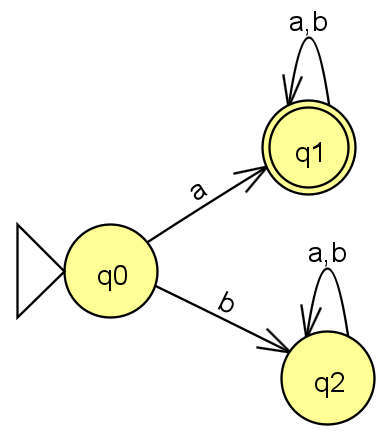
\includegraphics[width=0.2\textwidth]{../../../images/DFAs/ex1_q1.png}



% \vspace{3cm}
% \begin{flushleft}
% أرجو لكم وقتًا ممتعًا.

% الأستاذ محمود اغبارية.
% \end{flushleft}


% \end{document}


\ifwithsols
\title{حل وظيفة 9: آلة تورينج}
\else
\title{وظيفة 9: آلة تورينج}
\fi

\begin{document}

\maketitle

\begin{enumerate}[itemsep=2em]
\item صمّم آلة تيورنج تتلقى عددًا صحيحًا موجبًا $x$ على الشريط بالتمثيل الأوناري، وتحسب $x \% 3$، وتكتب النتيجة بالتمثيل الأوناري بين إشارتَي $\$$ في مكانٍ ما على الشريط.
\textbf{مثال} إذا كان المدخل هو: $11111$ (أي $x=5$)، فيجب أن تكتب الآلة $\$11\$$ (أي $5 \% 3 = 2$) في مكانٍ ما على الشريط.

\textbf{المدخل ($x=5$):}
\begin{tikzpicture}[scale=0.85]
    \foreach \i/\c in {1/$\vdash$,2/1,3/1,4/1,5/1,6/1,7/$\triangle$} {
        \draw (\i,0) rectangle +(1,0.8);
        \node at (\i+0.5,0.4) {\c};
    }
    \node at (8.5, 0.4) {$\ldots$};
\end{tikzpicture}

\vspace{0.5em}

\textbf{الناتج ($5 \% 3 = 2$):}
\hspace{0.5em}
\begin{tikzpicture}[scale=0.85]
    \foreach \i/\c in {1/$\vdash$,2/$\ldots$,3/$\$$,4/1,5/1,6/$\$$,7/$\ldots$} {
        \draw (\i,0) rectangle +(1,0.8);
        \node at (\i+0.5,0.4) {\c};
    }
\end{tikzpicture}

\ifwithsols
\begin{boxSolution}
\begin{center}
    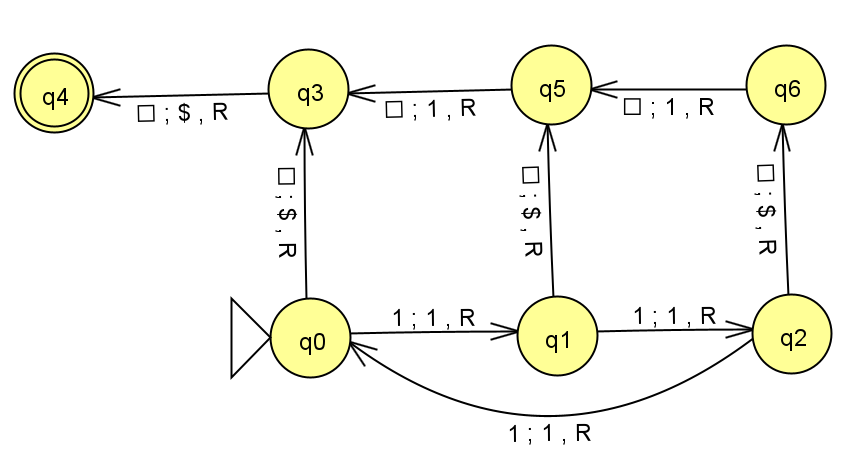
\includegraphics[width=0.4\paperwidth,keepaspectratio]{../../../images/turing/fx_xMod3.png}%
\end{center}
\end{boxSolution}
\fi

\ifwithsols
\else
\item السؤال الثاني في الصفحة التالية - المطلوب حل أول 3 بنود فقط، والبند الرابع اختياريّ.
\fi

\end{enumerate}

\ifwithsols
\else
\clearpage
\fi

\subsection*{سؤال 11 امتحان 899271 سنة 2024}
\addcontentsline{toc}{subsection}{سؤال 11 امتحان 899271 سنة 2024}

\noindent
\makebox[\textwidth][c]{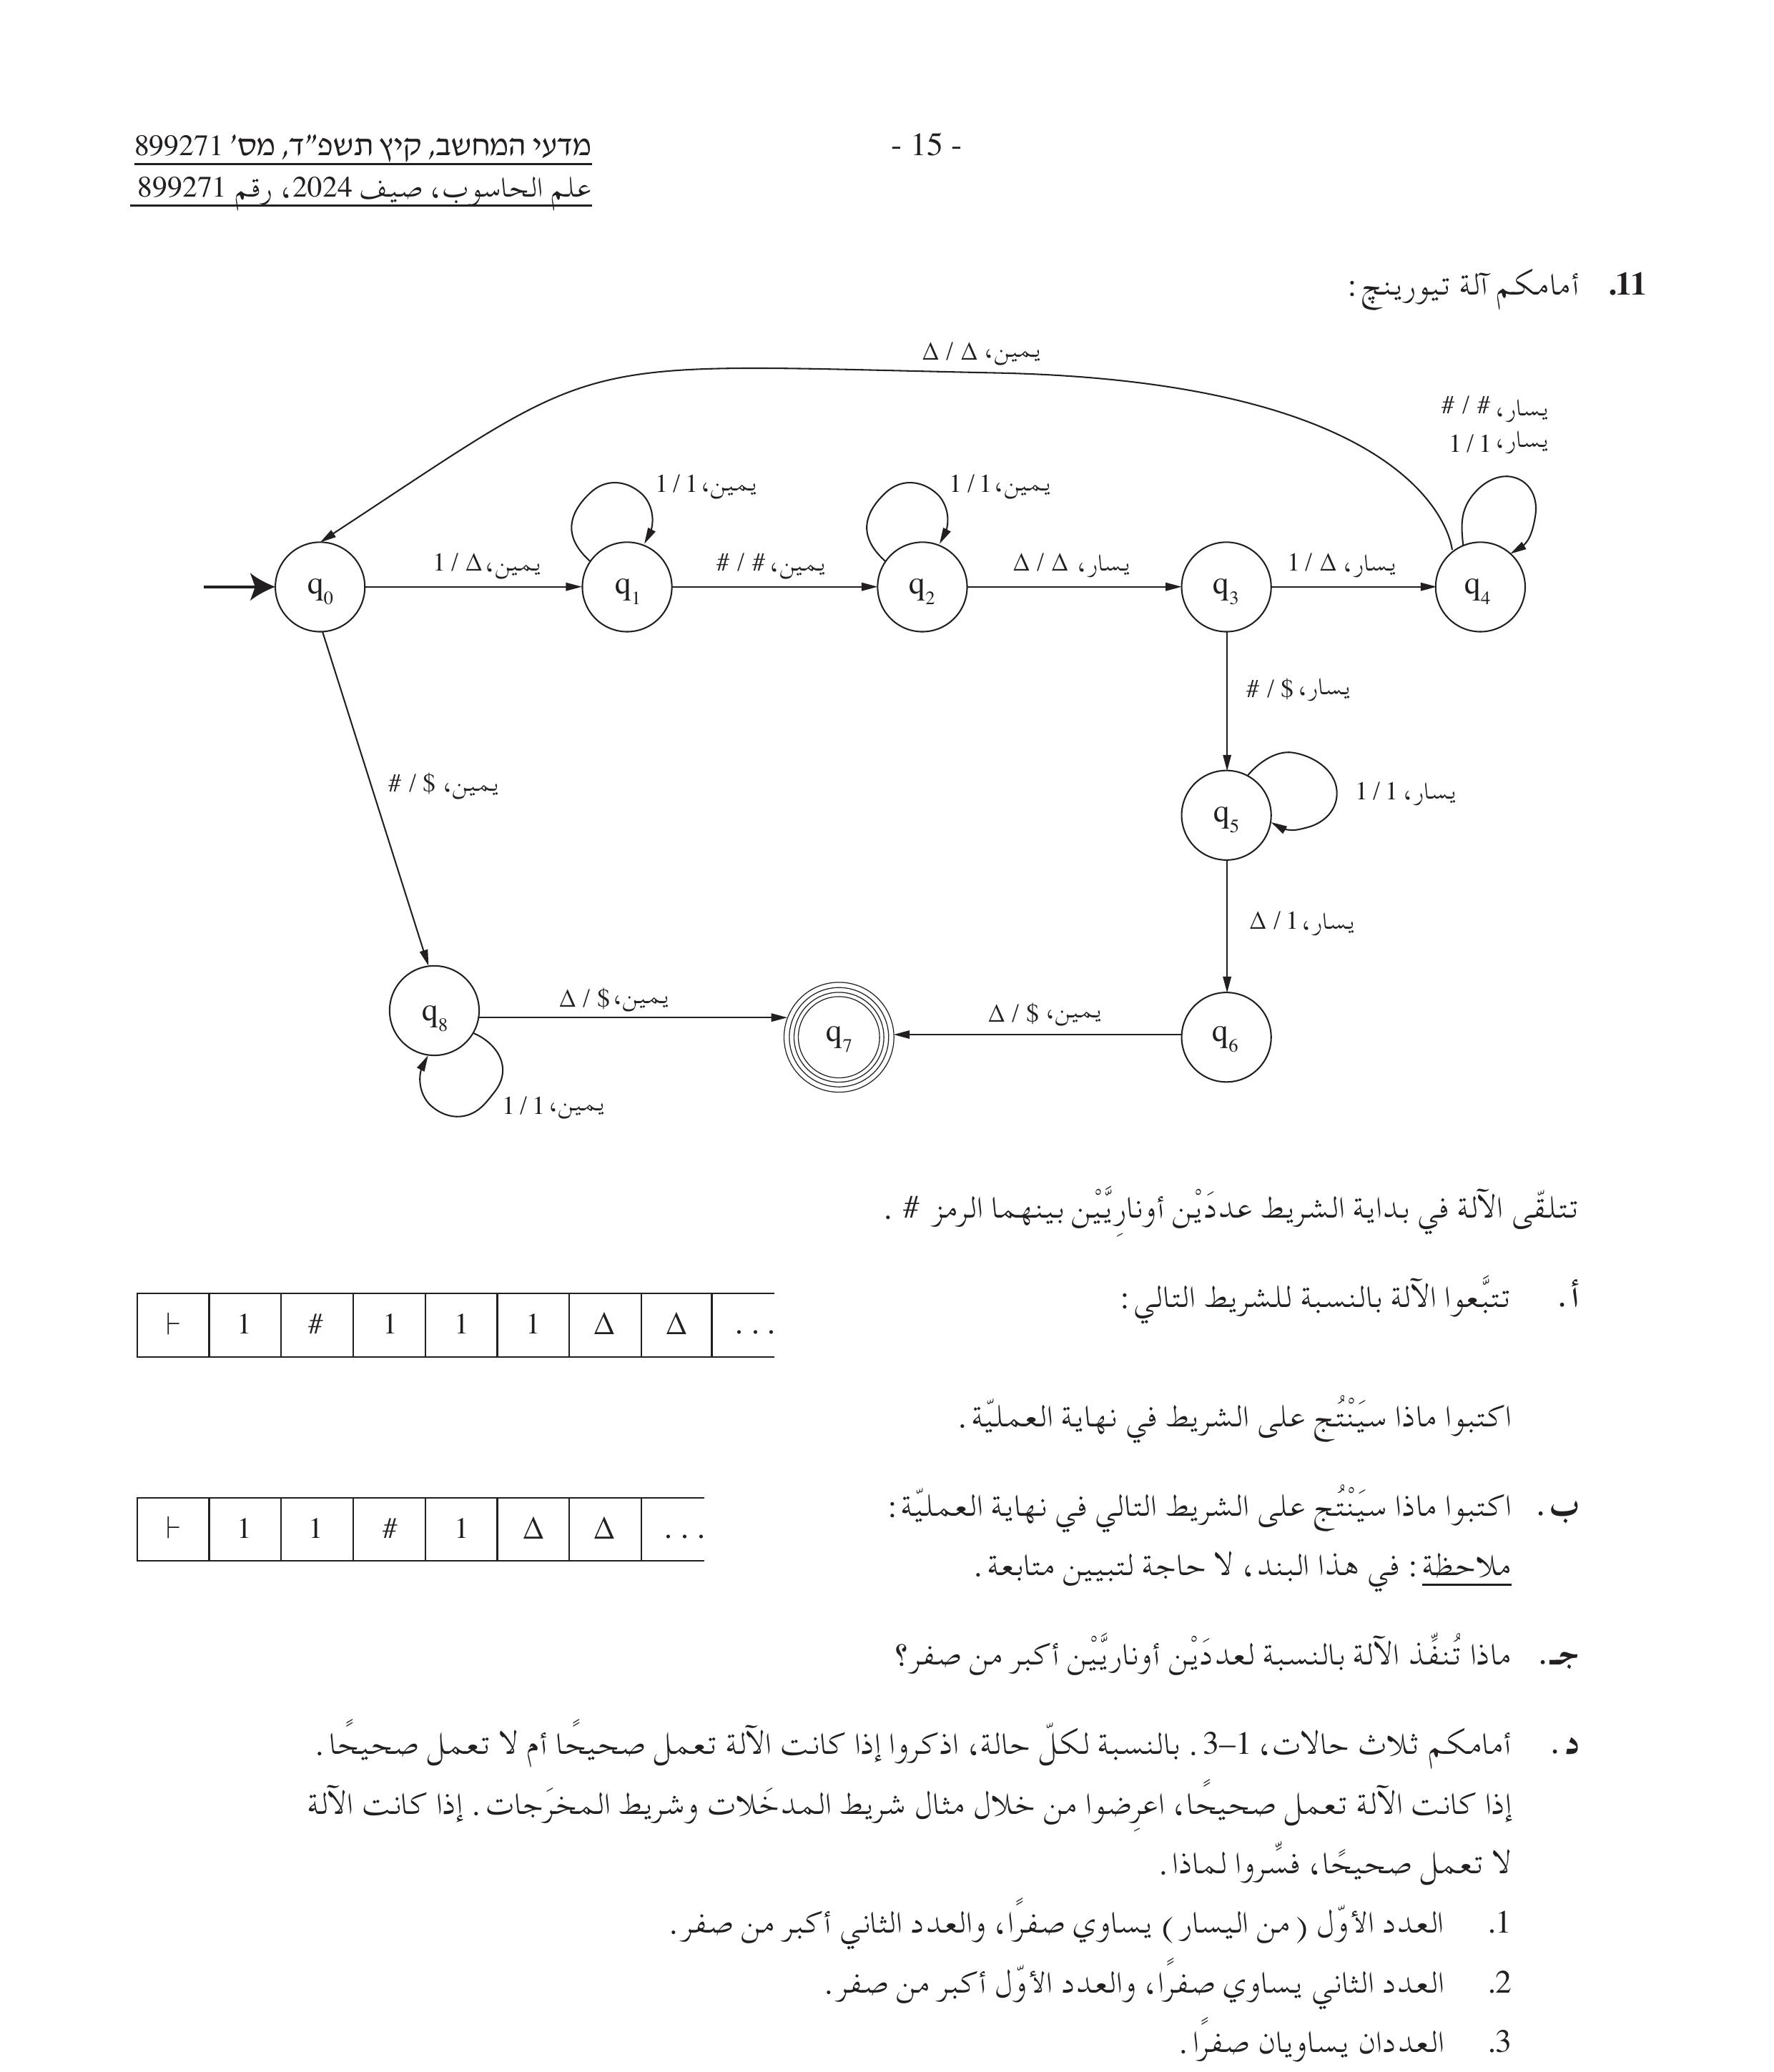
\includegraphics[width=0.9\paperwidth,keepaspectratio]{ ../../../bagrut_questions/computational_models/turing_2024_899271_11.jpg }%
}%

\ifwithsols
\begin{boxSolution}[سؤال 11 امتحان 899271 سنة 2024]
\begin{enumerate}[itemsep=1.5em, label=\alph*.]

\item
\textbf{المدخل ($x=1, y=3$):}
\hfill
\begin{tikzpicture}[scale=0.83]
    \foreach \i/\c in {1/$\vdash$,2/1,3/\#,4/1,5/1,6/1,7/$\triangle$,8/$\triangle$} {
        \draw (\i,0) rectangle +(1,0.8);
        \node at (\i+0.5,0.4) {\c};
    }
    \node at (9.5, 0.4) {$\ldots$};
\end{tikzpicture}

\textbf{تتبع الحالات:}
{\small
\begin{align*}
q_0 \quad &\vdash \; \underline{1} \; \# \; 1 \; 1 \; 1 \; \triangle \\
q_1 \quad &\vdash \; \triangle \; \underline{\#} \; 1 \; 1 \; 1 \; \triangle \quad \text{(مسح 1 من $x$، يمين)} \\
q_2 \quad &\vdash \; \triangle \; \# \; \underline{1} \; 1 \; 1 \; \triangle \\
q_2 \quad &\vdash \; \triangle \; \# \; 1 \; \underline{1} \; 1 \; \triangle \\
q_2 \quad &\vdash \; \triangle \; \# \; 1 \; 1 \; \underline{1} \; \triangle \\
q_2 \quad &\vdash \; \triangle \; \# \; 1 \; 1 \; 1 \; \underline{\triangle} \quad \text{(تجاوز العدد الثاني)} \\
q_3 \quad &\vdash \; \triangle \; \# \; 1 \; 1 \; \underline{1} \; \triangle \quad \text{(رأى $\triangle$، رجع يسارًا)} \\
q_4 \quad &\vdash \; \triangle \; \# \; 1 \; \underline{1} \; \triangle \; \triangle \quad \text{(مسح 1 من $y$، رجع يسارًا)} \\
q_4 \quad &\vdash \; \triangle \; \# \; \underline{1} \; 1 \; \triangle \; \triangle \\
q_4 \quad &\vdash \; \triangle \; \underline{\#} \; 1 \; 1 \; \triangle \; \triangle \\
q_4 \quad &\vdash \; \underline{\triangle} \; \# \; 1 \; 1 \; \triangle \; \triangle \\
q_0 \quad &\vdash \; \triangle \; \underline{\#} \; 1 \; 1 \; \triangle \; \triangle \quad \text{(رأى $\triangle$، تقدم يمينًا لدورة جديدة)} \\
q_8 \quad &\vdash \; \triangle \; \$ \; \underline{1} \; 1 \; \triangle \; \triangle \quad \text{($q_0$ يرى $\#$: انتهى $x$، كتب $\$$، يمين)} \\
q_8 \quad &\vdash \; \triangle \; \$ \; 1 \; \underline{1} \; \triangle \; \triangle \\
q_8 \quad &\vdash \; \triangle \; \$ \; 1 \; 1 \; \underline{\triangle} \; \triangle \quad \text{(تجاوز المتبقي من $y$)} \\
q_7 \quad &\vdash \; \triangle \; \$ \; 1 \; 1 \; \$ \; \underline{\triangle} \quad \text{(كتب $\$$ النهائية وتوقف للقبول)} \checkmark
\end{align*}
}

\textbf{ماذا سينتج على الشريط في نهاية العمليّة:}
\begin{tikzpicture}[scale=0.83]
    \foreach \i/\c in {1/$\vdash$,2/$\triangle$,3/\$,4/1,5/1,6/\$,7/$\triangle$,8/$\triangle$} {
        \draw (\i,0) rectangle +(1,0.8);
        \node at (\i+0.5,0.4) {\c};
    }
    \node at (9.5, 0.4) {$\ldots$};
\end{tikzpicture}
\\
$\leftarrow$ الناتج بين الـ\$: $1\,1$ (= 2 = |1 - 3|) \checkmark \\

\end{enumerate}
\end{boxSolution}

\begin{boxSolution}
\begin{enumerate}[itemsep=1.5em, label=\alph*., resume]
\item
المدخل هو $x=2, y=1$. بعد تكرار نفس العملية، سينتج على الشريط:

\hfill
\begin{tikzpicture}[scale=0.83]
    \foreach \i/\c in {1/$\vdash$,2/$\triangle$,3/\$,4/1,5/\$,6/$\triangle$,7/$\triangle$} {
        \draw (\i,0) rectangle +(1,0.8);
        \node at (\i+0.5,0.4) {\c};
    }
    \node at (8.5, 0.4) {$\ldots$};
\end{tikzpicture}
\\
$\leftarrow$ الناتج بين الـ\$: $1$ (= 1 = |2 - 1|) \checkmark \\

\item
تقوم الآلة بحساب \textbf{القيمة المطلقة للفرق بين العددين} $f(x,y) = |x - y|$. وتقوم بوضع الناتج النهائي محصوراً بين رمزي $\$$ الأولى و$\$$ الثانية.

\item
\begin{enumerate}
    \item \textbf{العدد الأول يساوي صفرًا، والعدد الثاني أكبر من صفر (مثال $x=0, y=2$):} \\
    \textbf{حالة الآلة:} تعمل صحيحًا. \\
    \textbf{التفسير:} تبدأ الآلة بقراءة $\#$ وتحوله إلى $\$$ وتنتقل إلى الحالة $q_8$. ثم تتخطى الآحاد يميناً، وعندما تقرأ الفراغ $\triangle$ تكتب $\$$ وتتوقف بنجاح في حالة القبول $q_7$.

    {\small
    \textbf{شريط المدخلات:}
    \hfill
    \begin{tikzpicture}[scale=0.83]
        \foreach \i/\c in {1/$\vdash$,2/\#,3/1,4/1,5/$\triangle$} {
            \draw (\i,0) rectangle +(1,0.8);
            \node at (\i+0.5,0.4) {\c};
        }
    \end{tikzpicture}

    \textbf{شريط المخرجات:}
    \hfill
    \begin{tikzpicture}[scale=0.83]
        \foreach \i/\c in {1/$\vdash$,2/\$,3/1,4/1,5/\$} {
            \draw (\i,0) rectangle +(1,0.8);
            \node at (\i+0.5,0.4) {\c};
        }
    \end{tikzpicture}
    }

    \item \textbf{العدد الثاني يساوي صفرًا، والعدد الأول أكبر من صفر (مثال $x=1, y=0$):} \\
    \textbf{حالة الآلة:} \underline{لا} تعمل صحيحًا. \\
    \textbf{التفسير:} بعد مسح الآحاد من العدد الأول (تصبح $\triangle$)، تصل الآلة لـ $\#$ وتستبدله بـ $\$$ في الحالة $q_3$ وتنتقل يساراً للحالة $q_5$. تقرأ الفراغ $\triangle$ وتستبدله بـ $1$ وتتحرك يساراً إلى الحالة $q_6$. في هذه اللحظة، سيصطدم رأس الآلة ببداية الشريط $\vdash$. نظرًا لأن الحالة $q_6$ غير معرّفة للتعامل مع الرمز $\vdash$، تتوقف الآلة قسرياً بشكل غير طبيعي (Crash) ولا تصل لحالة القبول.

    \item \textbf{العددان يساويان صفرًا ($x=0, y=0$):} \\
    \textbf{حالة الآلة:} تعمل صحيحًا. \\
    \textbf{التفسير:} تقرأ الآلة $\#$ وتحوله إلى $\$$ وتنتقل للحالة $q_8$. ثم تقرأ الفراغ $\triangle$ مباشرةً وتكتب $\$$ وتتوقف بنجاح في حالة القبول $q_7$.

    {\small
    \textbf{شريط المدخلات:}
    \hfill
    \begin{tikzpicture}[scale=0.83]
        \foreach \i/\c in {1/$\vdash$,2/\#,3/$\triangle$,4/$\triangle$} {
            \draw (\i,0) rectangle +(1,0.8);
            \node at (\i+0.5,0.4) {\c};
        }
    \end{tikzpicture}

    \textbf{شريط المخرجات:}
    \hfill
    \begin{tikzpicture}[scale=0.83]
        \foreach \i/\c in {1/$\vdash$,2/\$,3/\$,4/$\triangle$} {
            \draw (\i,0) rectangle +(1,0.8);
            \node at (\i+0.5,0.4) {\c};
        }
    \end{tikzpicture}
    }
\end{enumerate}

\end{enumerate}
\end{boxSolution}

\clearpage
\fi


\end{document}
